\documentclass[tikz]{standalone}

\begin{document}
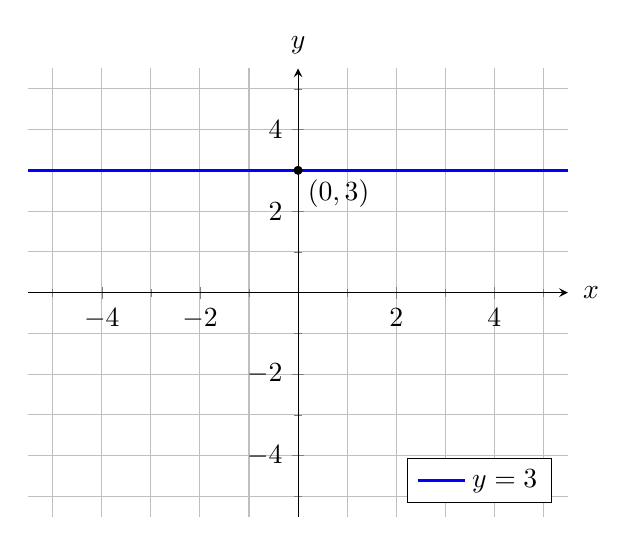
\begin{tikzpicture}
    \begin{axis}[%
        xlabel=$x$, ylabel=$y$, legend pos=south east,
        grid=both, xmin=-5.5, xmax=5.5, ymin=-5.5, ymax=5.5,
        axis lines = middle,
        minor x tick num=1, minor y tick num=1,
        xlabel style = {at={(axis description cs:1.01,0.5)},anchor=west},
        ylabel style = {at={(axis description cs:0.5,1.01)},anchor=south},
    ]
    \addplot+[blue, very thick, mark=none, domain=-5.5:5.5] plot {3};
    \addlegendentry{$y=3$}
    \draw[black, fill=black] (0,3) circle [radius=.5mm]
        node[below right]{$(0,3)$};
    \end{axis}
\end{tikzpicture}
\end{document}
